\documentclass[12pt]{article}
\usepackage{lingmacros}
\usepackage{tree-dvips}
\usepackage[utf8]{inputenc}
\usepackage[russian]{babel}
\usepackage{amsmath,amssymb}
\usepackage{multirow}
\usepackage{hyperref}
\usepackage{caption}

\usepackage{graphicx}
\graphicspath{ {./images/} }

\usepackage{listings}
\usepackage{color}

\definecolor{dkgreen}{rgb}{0,0.6,0}
\definecolor{gray}{rgb}{0.5,0.5,0.5}
\definecolor{mauve}{rgb}{0.58,0,0.82}
\definecolor{orange}{rgb}{1,0.6,0}

\lstset{frame=tb,
  language=C++,
  aboveskip=1mm,
  belowskip=1mm,
  showstringspaces=false,
  columns=flexible,
  basicstyle={\small\ttfamily},
  numbers=none,
  numberstyle=\color{orange},
  keywordstyle=\color{blue},
  commentstyle=\color{dkgreen},
  stringstyle=\color{mauve},
  breaklines=true,
  breakatwhitespace=true,
  tabsize=3
}

\begin{document}
\title{Lowest Common Ancestor. Sprase Table}
\date{}
\maketitle

\section*{Дефиниция и примери}
\subsection*{Дефиниция}
\paragraph*{}
Нека имаме кореново дърво $T$ с корен $root$. Връх $u$ се нарича предшественик на връх $v$, ако $u$ лежи на единствения път между $root$ и $v$. Ще бележим с $depth(u)$ дълбочината на връх $u$ или с други думи казано - разстоянието от $root$ до $u$. При тази конвенция, най-близкият общ предшественик на $u$ и $v$, който ще бележим с $lca(u, v)$, ще бъде върхът $x$ с максимална дълбочина, който е предшественик едновременно на $u$ и $v$. 
\subsection*{Примери}
\paragraph*{}
В този случай коренът е връх 1.

\begin{figure}[h]
\caption*{Фигура 1}
\centering
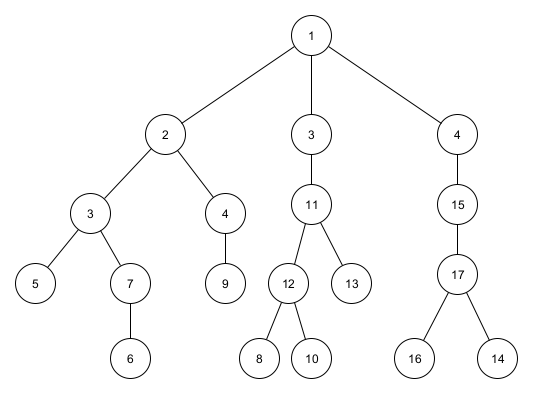
\includegraphics[width=0.5\textwidth]{tree1}
\end{figure}

\raggedright
\begin{itemize}
	\item $lca(5, 7) = 3$;
	\item $lca(4, 9) = 4$;
	\item $lca(3, 9) = 2$;
	\item $lca(2, 13) = 1$;
	\item $lca(4, 14) = 4$;
	\item $lca(2, 4) = 1$;
\end{itemize}

\section*{Свойства на lca(u, v)}
\begin{itemize}
	\item $lca(u, v) = lca(v, u)$
	\item $lca(u, v) = u$ тогава и само тогава, когато u e предшественик на $v$
	\item $lca(u, lca(v, w)) = lca(lca(u, v), w)$.
\paragraph*{}
По тази причина можем да записваме обобщено $lca(u, v, w)$. Това е полезно, ако например имаме нужда да пресмятаме $lca$ на цели интервали от масив. Поради това свойство знаем, че задачата има смисъл и може да се реши със сегментно дърво. От следващото свойство ще научим, че има и по-добър начин.
	\item $lca(u, v, v) = lca(u, v)$
\paragraph*{}
Това значи, че добавянето на "излишни" върхове към тези, на които търсим $lca$ не променя отговора. Тост ако искаме да сметнем $lca$ на група върхове можем да си ползволим да сметнем $lca$ на група, която съдържа тези върхове, но по няколко пъти. Това ни дава възможност да пресмятаме $lca$ на интервал от върхове чрез sparse table. Повече по темата ще научите по-късно.
	\item $lca(u, v) = lca(u, v')$, където $v'$ се получава, когато "качим" връх $v$ на нивото на връх $u$ (разбира се, приемаме, че $depth(u) \leq depth(v)$)
	\item $depth(lca(u, v)) \leq depth(u)$ и $depth(lca(u, v)) \leq v$.
\paragraph*{}
Можете да се убедите с примери от Фигура 1:
\begin{itemize}
	\item u = 5, v = 6, v' = 7
	\item u = 2, v = 13, v' = 3
	\item u = 11, v = 14, v' = 15
	\item u = 2, v = 9, v' = 2
\end{itemize} 
Тук ще покажем не съвсем формално доказателство на свойството. Ясно е, че след като само "покачваме" връхове то няма как $lca$ да "слезе". Затова само трябва да проверим, че $lca(u, v)$ е предшественик на $u$ и $v'$. Нека запишем $l = lca(u, v)$, тривиално е, че $l$ предшества $u$. Сега трябва да видим дали предшества $v'$. Допускаме противното: нека $l$ не предшества $v'$. Ние знаем, че $l$ предшества $v$. Тъй като ние само сме се качвали нагоре, то единственият вариант $l$ вече да не предшества $v'$ е да сме го "подминали", тоест $l$ да лежи на пътя между $v$ и $v'$. Ясно е също и че $l \neq v'$. Това обаче е противоречие, понеже $depth(l) \leq depth(u) = depth(v') \leq depth(v)$ и излиза, че няма как $l$ да лежи на пътя между $v$ и $v'$.
\end{itemize}

\section*{LCA с binary lifting}
\paragraph*{}
Използвайки тези свойства можем да изготвим алгоритъм, който намира $lca(u, v)$ за $O(logN)$. 
\paragraph*{}
Забелязваме, че ако имаме два върха $u$ и $v$ на равна дълбочина, то ако започнем постепенно да ги "качваме" едновременно, то стойностите ще се различават до един момомент и по-конкретно, първата стойност на съвпадение ще бъде точно $lca(u, v)$. Нека имаме функция $rise(u, n)$, която връща връх, отговарящ на връх $u$ след като бъде "качен" с $n$ стъпки. Тоест така излиза, че трябва да намерим най-малкото $n$, за което $rise(u, n) = rise(v, n)$ и тази стойност ще бъде $lca(u, v)$. По-късно обаче, ще стане ясно, че е по-добре да намерим последното $n$, за което $rise(u, n) \neq rise(v, n)$ и така $lca(u, n)$ ще бъде $parent(rise(u, n))$, където $paret(x)$ е родителят на $x$.
\paragraph*{}
От тези наблюдения става ясно, че е доста удобно да имаме бърз начин да "качваме" връхове. По тази причина е измислена техниката binary lifting. Идеята е следната: за всеки връх $x$ пазим $rise(x, 1)$, $rise(x, 2)$, $rise(x, 4)$, ..., $rise(x, 2^k)$, ... (разбира се няма нужда да пазим тези стойности до безкрай, а само до достатъчно голяма степен на 2). Ключовото наблюдение тук е, че тези стойности могат да се пресмятат доста лесно. Например: $rise(x, 1) = parent(x)$. Също така $rise(x, 2) = parent(parent(x)) = rise(rise(x, 1), 1)$. Забелязваме също и че: $rise(x, 2^k) = rise(rise(x, 2^{k-1}), 2^{k-1})$. Това е вярно, понеже искаме да направим $2^k$ стъпки нагоре, които можем да разделим на два скока по $2^{k-1}$. Разбира се, че ако се опитаме да скочим прекалено нагоре, няма да има връх в дървото, който да отговаря на този скок. Например $rise(2, 2)$ в дървото от Фигура 1 не съществува. Затова за такива случаи записваме, че стойността е $-1$. Също така приемаме, че $rise(-1, 2^k) = -1$.  Сега можем да разширим способностите на нашата функция $rise$. Забелязваме, че ако можем да представим число като сума от степени на двойката, то можем и да направим подходяща поредица от изкачвания, с които да постигнем скок с исканата големина. Например, ако искаме да пресметнем $rise(x, 7)$ можем да използваме $rise(rise(rise(x, 1), 2), 4)$. Тоест, като използваме, че $7=4+2+1$, то правим първо скок с дължина 1, после скок с дължина 2 и накрая скок с дължина 4. Друг пример е: $rise(x, 10) = rise(rise(x, 2), 8)$.
\paragraph*{}
Имайки тези знания можем да направим алгоритъм, който може да намира $lca$ на два върха $u$ и $v$. Допускаме, че $dept(u) \leq depth(v)$. Първо можем да изравним дълбочината на двата върха за $O(logN)$ и така ще трябва да смятаме $lca$ на два върха с еднаква дълбочина. Нека новата стойност на $v$ след изравняването бъде $v'$. Тогава знаем, че същестува $n$, за което $rise(u, n) \neq rise(v', n)$ и $rise(u, n+1) = rise(v', n+1)$. Тоест искаме да намерим последното $n$, за което някакво си условие е в сила. В такива ситуации можем да направим нещо като binary search по битовете на $n$ и да се опитваме да правим старши битове да бъдат $1$ без да разваляме свойството. По-конкретно, тръгваме да ходим по битовете на числото в обратен ред $MAXBit, MAXBit-1, MAXBit-2, ..., 2, 1, 0$ и за всеки бит $b$ проверяваме дали $rise(u, n+2^b) \neq rise(v', n+2^b)$, ако да, то $n += 2^b$ ($n$ започва от $0$). За повече детайли вижте имплементацията.  	

\subsection*{Имплементация}
\paragraph*{}
Имплементацията на lca with bynary lifting е също доста проста, както и идеята. Грубо казано, след като имаме определен корен на дървото ще пуснем едно $dfs$, което да инициализира родителите и дълбочините на върховете. Също трябва да попълним стойностите за скоковете нагоре в дървото, което може да се направи лесно, ако ги пазим в таблица. Тук е изложена и примерна имплементация.  

\begin{lstlisting}
#include <iostream>
#include <vector>

using namespace std;

const int MAXN = 1e5;
const int MAXLog = 20;

int n;
vector <int> graph[MAXN];

int parent[MAXN], depth[MAXN];
int sparse[MAXLog+2][MAXN];

void dfs(int x, int last, int level)
{
    parent[x] = last;
    depth[x] = level;

    for(int y: graph[x])
    {
        if(y!=last)
            dfs(y, x, level+1);
    }
}

void init(int root)
{
    dfs(root, -1, 1);
    for(int x = 1;x<=n;x++) sparse[0][x] = parent[x];

    for(int l = 1;l<=MAXLog;l++)
    {
        for(int x = 1;x<=n;x++)
        {
            if(sparse[l-1][x]==-1)
                sparse[l][x] = -1;
            else
                sparse[l][x] = sparse[l-1][sparse[l-1][x]];
        }
    }
}

int rise(int x, int levelDiff)
{
    for(int bit = 0;bit<=MAXLog;bit++)
    {
        if(((levelDiff>>bit)&1)==1)
        {
            if(x!=-1)
                x = sparse[bit][x];
        }
    }

    return x;
}

int lca(int u, int v)
{
    if(depth[u]>depth[v])
        swap(u, v);

    v = rise(v, depth[v]-depth[u]);
    if(u==v) return u;

    for(int l = MAXLog;l>=0;l--)
    {
        if(sparse[l][u]!=sparse[l][v])
        {
            u = sparse[l][u];
            v = sparse[l][v];
        }
    }

    return parent[u];
}

int main()
{
    cin >> n;
    for(int i = 0;i<n-1;i++)
    {
        int a, b;
        cin >> a >> b;

        graph[a].push_back(b);
        graph[b].push_back(a);
    }

    int root;
    cin >> root;

    init(root);
}

\end{lstlisting}

\section*{Приложение на LCA}
\subsection*{Пътища в дърво}
\paragraph*{}
Единственият път от $u$ до $v$ в дърво е точно пътят $u \rightarrow lca(u, v) \rightarrow v$. Тоест от $u$ се качваме до $lca(u, v)$ и след това от там слизаме до $v$. 
\subsection*{Проверка за положение на върхове}
\paragraph*{}
Можем да проверим дали връх $u$ e предшественик на връх $v$, ако проверим дали $lca(u, v)$ е равно на $u$.

\section*{Задачи за LCA}
\subsection*{Открито първенство на София по информатика - В2 Пътища}
\paragraph*{}
\href{https://arena.olimpiici.com/#/catalog/533/problem/1326}{Условие на задачата} 

\subsection*{Codeforces - Hill Climbing}
\paragraph*{}
\href{https://codeforces.com/problemset/problem/406/D}{Условие на задачата}

\end{document}